\documentclass[a4paper,10pt]{article}

\usepackage{float}
\usepackage{amsmath}
\usepackage{style}
\usepackage{makeidx}
\usepackage{color}
\setlength{\parindent}{15pt}
\usepackage{pdfpages}
\usepackage[abs]{overpic}
\setlength\unitlength{1mm}

\title{Laboration 2 - Svängningar \\ Fysik - Mekanik och vågor (FAFA01)}
\author{Björn Wictorin, bjorn.wictorin@gmail.com \\ Patrik Laurell, patrik.laurell@gmail.com \\ \\ Handledare: Magnus Dagbro}
\date{Utförandedatum: 31 mars 2014 \\ Inlämingsdatum: \today}

\begin{document}


\maketitle
\thispagestyle{empty}
\newpage
\pagenumbering{roman}
\tableofcontents{}
\pagebreak

\pagenumbering{arabic}

\section{Inledning}
Många fysikaliska fenomen kan beskrivas med hjälp av oscillerande system. Exempel på sådana fenomen är fjädrar, pendlar och spänningar i LCR-kretsar. Syftet med denna laboration var att ge en bättre förståelse för de modeller som används för att beskriva olika typer av oscillerande system. Vidare gav laborationen ökad träning i användning av datorprogrammen DataStudio för insamling av mätdata och Matlab för analysering av dessa. Laborationen gav också övning i att använda ett oscilloskop.

\section{Teori}
Modellen för ett oscillerande system beskriver ett system i vilket nettokraften på ett objekt verkar för att återföra det till ett stabilt jämviktsläge. Således kan alla system av denna typ beskrivas som oscillerande. Exempel på sådana system är fjädrar som svänger och pendlar. Den återförande kraften är proportionell mot avståndet till jämviktsläget. Detta samband kan, om dämpande krafter försummas, uttryckas matematiskt med följande ekvation:
\begin{equation}
	F = -kx
\end{equation}
där $k$ är en systemberoende konstant och $x$ är avståndet till systemets jämviktspunkt. Ekvation (1) beskriver alltså en odämpad oscillerande rörelse och ur den kan ett samband för positionen av en partikel som funktion av tiden härledas. Detta ger följande ekvation:
\begin{equation}
	x(t) = A cos(\omega_0t + \delta)
\end{equation}
där $\omega_0$ är systemets s.k. egenvinkelfrekvens, $A$ är amplituden av svängningen och $\delta$ är fasförskjutningen. Egenvinkelfrekvensen är den vinkelfrekvens med vilken systemet svänger om det in påverkas av yttre krafter. \\
\indent Dock är sällan fallet i verkligheten att ett system är odämpat. Krafter från omgivningen dämpar ofta svängningar så att de bromsas. För att beskriva sådana fall används en modell för dämpad svängning. I denna modell antas den dämpande kraften vara proportionell mot hastigheten. Dämpade oscillationer kan beskrivas med följande ekvation:
\begin{equation}
	F = -kx - b\frac{dx}{dt} \Longleftrightarrow m\frac{d^2x}{dt^2} + b\frac{dx}{dt} + kx = 0
\end{equation}
Ekvation (3) beskriver en andra ordningens differentialekvation i $x$. Ur denna ekvation kan formler för tre olika typer av dämpade svängningar tas fram. Dessa är svagt dämpade, kritiskt dämpade eller överdämpade. I denna laboration ligger fokus på svagt dämpade svängningar. Dessa är de enda dämpade svängningar som ger upphov till en oscillerande rörelse. För en svagt dämpad svängning ges positionen som funktion av tiden av:
\begin{equation}
	x(t) = A_0e^{-\frac{b}{2m}t}\cos(\omega't + \delta))
\end{equation}
där $\omega'$ är den frekvens som systemet svänger med. $\omega'$ bestäms med ekvationen:
\begin{equation}
	\omega' = \sqrt{\omega_0^2-(\frac{b}{2m})^2}
\end{equation}
I ekvation (4) ser man att amplituden är exponentiellt avtagande. Den tid det tar för amplituden att minska till $\frac{1}{e}$ av utgångsamplituden kallas för systemets tidskonstant och betecknas $\tau$. Utifrån tidskonstanten kan även systemets halveringstid bestämmas.
\\
\indent För att en dämpad svängning inte ska stanna upp måste energi tillföras. Svängningar där energi tillförs kallas drivna svängningar. Ett svängande system kan vara både dämpat och drivet samtidigt. I modellen för ett dämpat och drivet system antas den drivande kraften vara periodisk och den dämpande proportionell mot hastigheten. Systemet beskrivs med differentialekvationen
\begin{equation}
F = -kx - b\frac{dx}{dt} + F_0\cos(\omega t) \Longleftrightarrow\frac{d^2x}{dt^2} + \frac{b}{m}\cdot\frac{dx}{dt} + \omega_0^2x = \frac{F_0}{m} \cos(\omega t)
\end{equation}
där $\omega$ är den vinkelfrekvensen med vilken den drivande kraften driver systemet.
Vilken påverkan den drivande kraften ha på systemet beror på hur $\omega$ förhåller sig  till systemets svängningsfrekvens $\omega'$. Lösningen till differentialekvationen är:
\begin{equation}
\begin{cases}
	x(t) = Acos(\omega t + \delta) \\
	A = \frac{F_0/m}{\sqrt{(\omega_0^2 - \omega^2)^2 + (\frac{b\omega}{m})^2}} \\
	\delta = \frac{\pi}{2} - \varphi \\
	tan(\varphi) = \frac{m(\omega_0^2 - \omega^2)}{b\omega}
\end{cases}
\end{equation}
där $A$ är amplituden för svängningen och $\delta$ är fasförskjutningen. Om den drivande frekvensen ligger nära $\omega'$ uppstår resonans, vilket innebär att energiöverföringen från den drivande kraften till systemet blir maximal. Detta ses ur lösningen till differentialekvationen. I ekvation (7) kan ses att ju närmre $\omega$ kommer $\omega_0$ desto större blir amplituden. Ekvationen för fasförskjutningen ger att $\delta \rightarrow \frac{\pi}{2}$ då $\omega \rightarrow \omega_0$. Vid resonans är alltså fasförskjutningen mellan den drivande kraften och systemets svängning $\frac{\pi}{2}$ radianer. För drivande frekvenser över resonansfrekvensen ligger $\delta$ mellan $\frac{\pi}{2}$ och $\pi$ radianer. Ju högre frekvensen blir, desto närmre $\pi$ går $\delta$. För drivande frekvenser under resonansfrekvensen ligger $\delta$ mellan $\frac{\pi}{2}$ och noll radianer. Ju lägre frekvensen blir, desto närmre kommer $\delta$ noll. Systemets svängning ligger i alla tre fallen efter den drivande kraftens svängning.\\
\indent I en elektrisk LCR-krets, dvs. en krets med spolar, kondensatorer och resistorer, uppstår svängningar i spänningen då kretsen matas med en fyrkantsvåg. Dessa svängningar utgör ett dämpad oscillerande system eftersom elektrisk energi går över till värmeenergi i kretsens resistor. Med ett oscilloskop kan dessa svängningar studeras. I fallet med en LCR-krets bestäms tidskonstanten med formeln: 
\begin{equation}
\tau = \frac{L}{R}
\end{equation}
Egenvinkelfrekvensen för en LCR-krets ges av:
\begin{equation}
\omega_0 = \frac{1}{\sqrt{LC}}
\end{equation}
denna frekvens är ej att blanda ihop med $\omega'$, vilket är frekvensen med vilken systemet kommer att svänga.

\pagebreak
\section{Apparatur}
Under laborationen användes följande apparatur:
\begin{itemize}
	\item Dator med Matlab och DataStudio
	\item Fjäder med vikt
	\item Ultraljudssensor
	\item Motor med reglerbart varvtal
	\item Vinkelgivare (Rotary Motion Sensor)
	\item Oscilloskop
	\item RCL-krets med trimpotentiometer
	\item Signalgenerator
\end{itemize}

\section{Utförande}
\subsection{Det dämpade men odrivna systemet}
Fjädern och vikten sattes i svängning och svängningen registrerades med ultraljudssensorn, samt plottades med DataStudio. I DataStudio bestämdes sedan systemets egenvinkelfrekvens $\omega'$. Ett fasdiagram, dvs. hastighet som funktion av läget, för systemet ritades sedan i DataStudio. Den insamlade datan flyttades sedan till Matlab för vidare analys. I Matlab subtraherades avståndet från sensorn till systemets jämviktsläge från alla mätvärden. Detta för att få positionen för svängningen relativt viloläget istället för relativt sensorn. I Matlab beräknades systemets hastigheten genom numerisk derivering av lägespositionerna. Sedan plottades $v^2$ och $\omega_0^2x^2$ och summan av dessa som funktioner av tiden. Ur diagrammet bestämdes systemets tidskonstant, samt halveringstiden för energin.

\subsection{Det drivna systemet}
Motorn sattes igång och fick driva fjädern. Motorns matningsspänning varierades, och på så sätt varierades även motorns varvtal och vinkelhastighet. Resonansvinkelfrekvensen söktes upp genom att den frekvens noterades för vilken systemet fick störst amplitud. Sedan studerades hur systemets fasförskjutning såg ut för drivfrekvenser över, på och under resonansfrekvensen.

\subsection{En LCR-krets}
En LCR-krets, dvs. en krets med en spole, en kondensator och en resistor kopplade i serie, var inkopplad till en funktionsgenerator. Funktionsgeneratorn ställdes in på att generera en fyrkantsvåg med frekvensen 200Hz. Oscilloskopets två kanaler kopplades in över signalgeneratorn och över kondensatorn.\\
\indent Resistansen varierades och spänningen över kondensatorn studerades då en svagt, kritiskt och överdämpad svängning uppstod. Den svagt dämpade svängningens frekvens bestämdes. Detta gjordes genom att tiden för ett antal perioder mättes upp med hjälp av oscilloskopets cursor-funktion. Periodtiden bestämdes genom att tiden dividerades med antalet perioder.\\
\indent Till sist bestämdes frekvensen genom att inversen till periodtiden togs fram. För den svagt dämpade signalen bestämdes också den exponentiella dämpningen. Detta gjordes genom att spänningsnivån bestämdes för den första vågtoppen samt för ytterligare en vågtopp. Tidsskillnaden mellan de båda vågtopparna mättes också upp. Utifrån dessa värden togs en exponentiellt avtagande funktion fram, från vilken tidskonstanten bestämdes.

\section{Resultat}
\subsection{Det dämpade men odrivna systemet}
Avståndet från ultraljudssensorn till fjäderns ändpunkt som funktion av tiden visas i figur 1. Utifrån denna data bestämdes systemet egenvikelfrekvens $\omega'$ till 3.46s\textsuperscript{-1}
\begin{figure}[H]
	\centering
	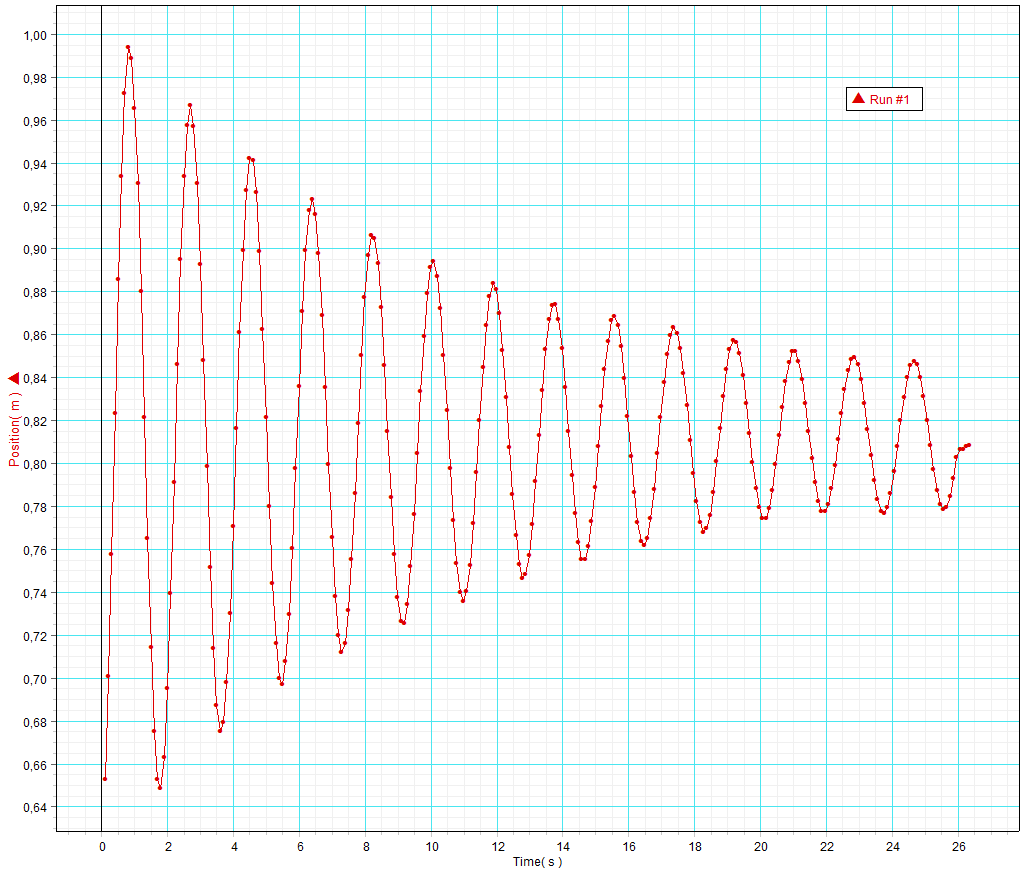
\includegraphics[width=0.8\textwidth]{../bilder/pos_vs_tid_uppg1.png}
	\caption{Position som funktion av tid.}
\end{figure}
Ett fasdiagram för systemets svängning visas i figur 2.
\begin{figure}[H]
	\centering
	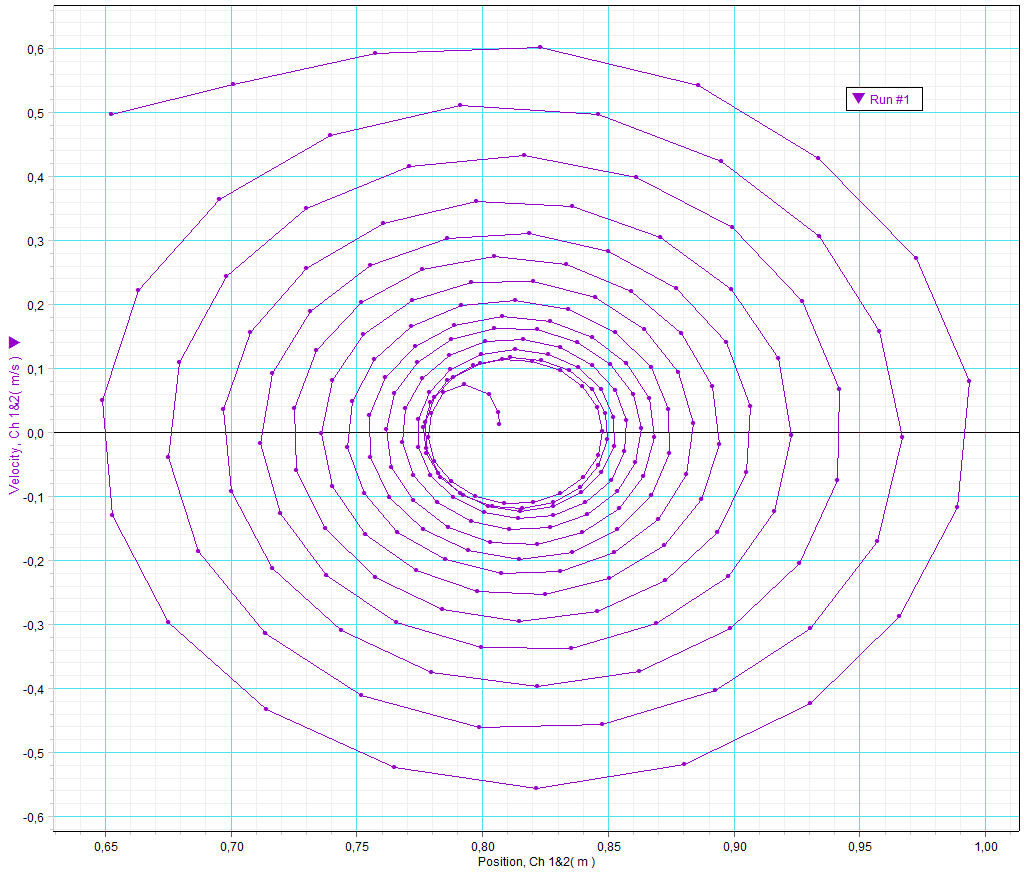
\includegraphics[width=0.8\textwidth]{../bilder/fasdiagram_uppg1.png}
	\caption{Svängningens hastighet som funktion av dess position.}
\end{figure}
I figur 3 visas förhållandet mellan läges- respektive rörelseenergin i systemet som funktion av tiden.
\begin{figure}[H]
	\centering
	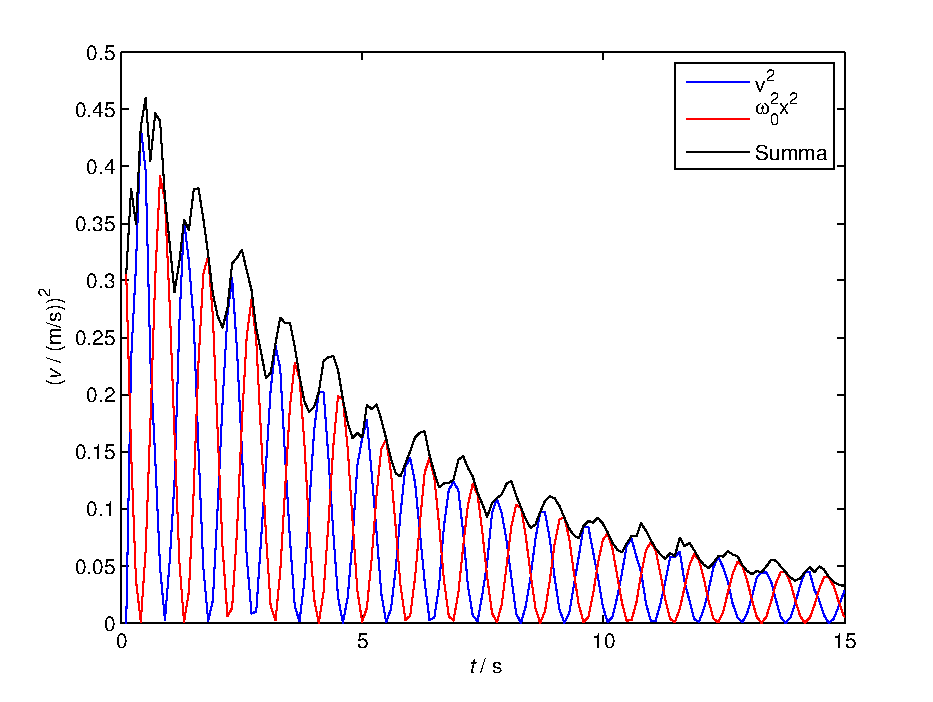
\includegraphics[width=0.8\textwidth]{../bilder/energigraf_uppg1.pdf}
	\caption{Här visas $v^2$, $\omega_0^2x^2$ samt summan av de båda som funktioner av tiden, där $v$ är svängningens hastighet.}
\end{figure}
Tidkonstanten för systemet bestämdes ur figur 3 till $\tau=4.94$s. Halveringstiden beräknades utifrån detta till 3.42s

\subsection{Det drivna systemet}
Genom iakttagande av systemet bestämdes resonansfrekvensen till $\omega=3.36$s\textsuperscript{-1}. I figur 4 visas position som funktion av motorns vinkelposition för drivande frekvenser vid resonans, under resonans samt över resonans.
\begin{figure}[H]
	\centering
	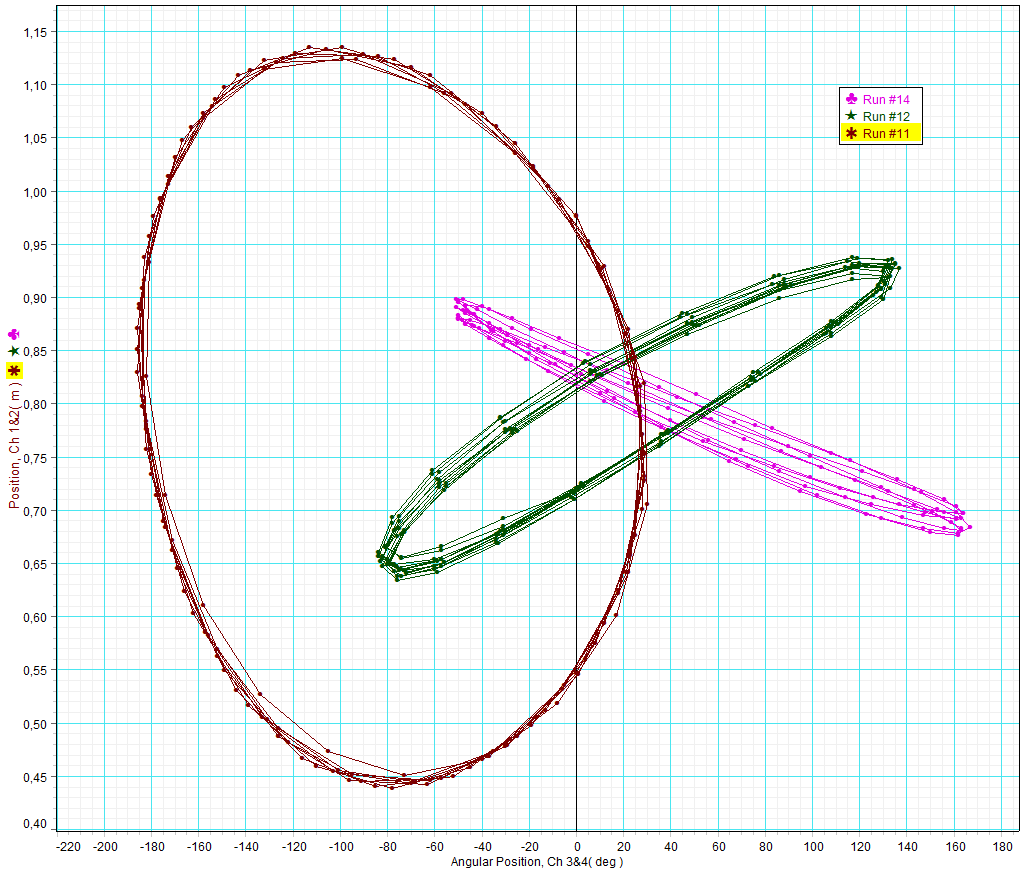
\includegraphics[width=0.8\textwidth]{../bilder/pos_vs_ang_uppg2b.png}
	\caption{Läget som funktion av vinkelposition för olika drivande frekvenser.}
\end{figure}
Då den drivande kraften hade en frekvens under resonansfrekvensen blev systemets fasförskjutning mindre än $\frac{\pi}{2}$ radianer, vilket syns på den gröna grafen i figur 4. Då drivfrekvensen motsvarade resonansfrekvensen var fasförskjutningen ungefär $\frac{\pi}{2}$ radianer. Detta syns i den röda grafen i figur 4. För frekvenser över resonansfrekvensen närmade sig fasförskjutningen $\pi$ radianer, vilket syns i den rosa grafen i figur 4. I samtliga tre fall var fasförskjutningen negativ relativt den drivande kraften.

\subsection{En LCR-krets}
Svängningens frekvens uppmättes till 2.3 kHz. Komponentvärdena för LCR-kretsen var 47mF för kondensatorn och 9 mH för spolen. Vid den svagt dämpade svängningen var trimpotentiometern inställd på 5.0$\Omega$. Spolen hade en inre resistans på 2.5$\Omega$. Den totala resistansen i kretsen var alltså 7.5$\Omega$. Tidskonstanten för svängningens exponentiella dämpning bestämdes till 0.96 ms.

\section{Diskussion}
\subsection{Det dämpade men odrivna systemet}
Systemets egenvinkelfrekvens uppmättes till 3,46 s\textsuperscript{-1}. Detta hade kunnat förändras genom att en vikt med en annan massa hängdes i fjädern eller genom att fjädern byttes ut mot en fjäder med en annan fjäderkonstant. Frekvensen hade också kunnat förändras genom att den bromsande kraften ökades, exempelvis genom att skivan i änden på fjädern gjordes mindre. Detta skulle nämligen minska luftmotståndet för svängningen.\\
\indent Att fasdiagrammet ser ut som en spiral beror på att amplituden för svängningen avtar efterhand som den bromsas ner. Samtidigt avtar då hastigheten eftersom frekvensen ska bevaras på samma nivå. Att spiralen går medurs beror på att fjädern har en negativ hastighet då den kommer från det positiva ändläget. Sedan har den en positiv hastighet när den kommer från det negativa ändläget. Man skulle alltså inte kunna ändra spiralen så att den gick moturs.
\begin{figure}[H]
\centering
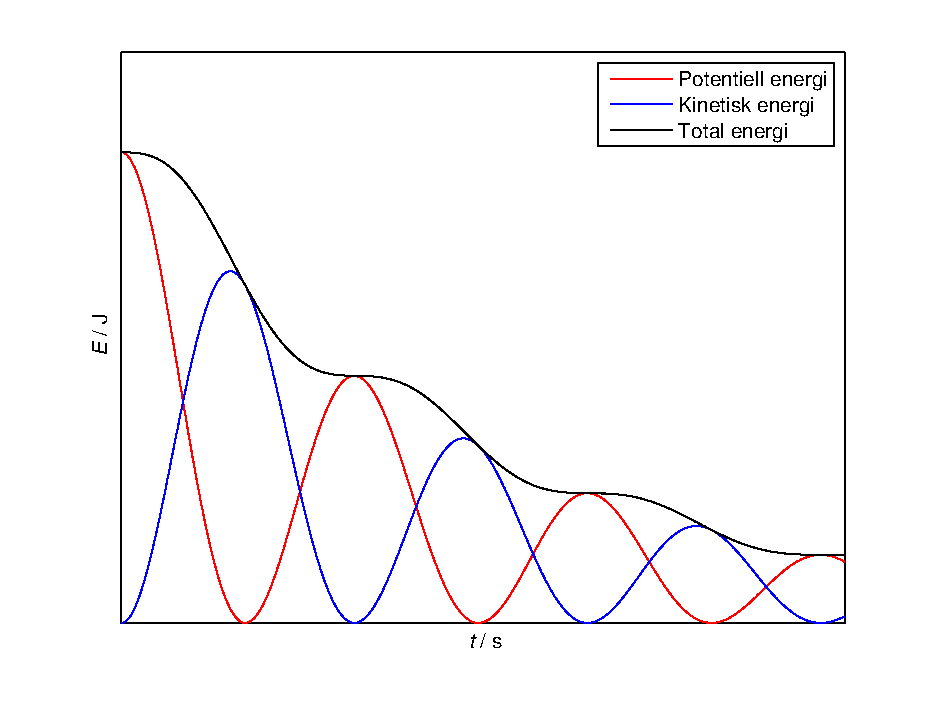
\includegraphics[width=0.8\textwidth]{../bilder/energigraf_uppg1_ideal.pdf}
\caption{Schematisk bild över hur energinivån i ett dämpat oscillerande system varierar över tiden. Bilden är genererad i Matlab.}
\end{figure}

Figur 5 visar en schematiskt bild över hur energinivån teoretiskt förändras i en dämpad svängning. Enligt teorin borde energidiagrammet i figur 3 se ut mer som det i figur 5. Den totala energin ska inte kunna öka vid något tillfälle, utan istället ska hastigheten med vilken den avtar variera. Störst är avtagandet kring jämviktsläget. Det beror på att svängningen har störst fart här. Stor fart medför stort luftmotstånd för plattan som är fäst vid fjäderns ände, eftersom luftmotståndet beror på hastigheten. Luftmotståndet är den största anledningen till att fjäderns rörelse dämpas. Att mätvärdena ger upphov till grafer så som de ser ut i figur 3 beror troligen på någon form av mätfel, t.ex. skulle det kunna vara så att ultraljudssensorn tar mätpunkter med för låg frekvens. Detta medför problem vid beräkningen av energinivåerna eftersom rörelseenergin beror på hastigheten, vilken tas fram med numerisk derivering. För få mätvärden ger försämrad numerisk derivering. Eftersom energin är proportionell mot hastigheten i kvadrat blir eventuella små fel förstorade.\\
\indent Ett annat problem vid mätningarna var att fjädern svängde en aning i sidled, vilket medförde att avståndet mellan plattan i fjäderns ände och sensorn inte varierade på riktigt samma sätt som fjäderns längd varierade då fjädern svängde.

\subsection{Det drivna systemet}
Den uppmätta resonansfrekvensen var 3.35 s\textsuperscript{-1}. Denna frekvens ligger nära systemvinkelfekvensen för det dämpade systemet, vilken låg på 3.46 s\textsuperscript{-1}. Eftersom resonans uppstår då den drivande kraftens frekvens ligger nära systemets vinkelfrekvens, stämde värdet på den observerade resonansfrekvensen väl överens med det förväntade.\\
\indent Figur 4 visar att systemets fasförskjutning för drivfrekvenser vid, över och under resonansfrekvensen stämde överens med teorin. Att plotten blev en cirkel då resonans uppstod visar att den drivande kraften och fjäderns rörelse låg $\frac{\pi}{2}$ radianer ur fas. Att det istället blev en ellips som lutar åt vänster då den drivande kraftens frekvens var större än resonansfrekvensen tyder på att fasförskjutningen närmade sig $\pi$ radianer. Hade den drivande frekvensen höjts upp så högt att fasförskjutningen faktiskt blev $\pi$ radianer skulle ellipsen bara bli en linje med negativ derivata. På samma sätt var det överensstämmande med teorin att det för drivande frekvenser under resonansfrekvensen blev en ellips lutande åt höger.

\subsection{En LCR-krets}
Som beskrivs i teoridelen kan LCR-kretsens svängningsfrekvens bestämmas utifrån komponentvärdena för spolen respektive kondensatorn. Den teoretiska svängningsfrekvensen blir utifrån dessa värden med hjälp av ekvation (9) till 2.44 kHz. Detta värde ligger nära det uppmätta värdet på 2.3 kHz.\\
\indent Enligt ekvation (8) i teorin är värdet på dämpningskonstanten $\tau = 1.2 $ ms. Detta ligger en bit över det värde erhölls från mätningarna, vilket var 0.96 s. Detta beror till största del på att resistansen i kretsen är större än det resistansvärde som $\tau$ beräknades utifrån. Då $\tau$ beräknades försummades nämligen resistansen i alla ledningar. Vid en ökning av resistansen ses i ekvation (8) att $\tau$ minskar. Att ta med kablarnas resistans i beräkningarna skulle alltså ge ett teoretiskt värde närmare det uppmätta. Vid en upprepning av laborationen hade det varit bra att mäta upp den faktiska resistansen i kretsen, för att kunna beräkna ett mer korrekt värde på $\tau$. Även komponentvärdena på spolen respektive kondensatorn kan ha avvikt något från de angivna värdena.\\
\indent En LCR-krets lämpar sig väl för att studera dämpade svängningar eftersom den dämpande kraften beror på resistansen, vilken är en faktor som kan kontrolleras och regleras noggrant.

\end{document}